\documentclass{report}

\usepackage[utf8]{inputenc}
\usepackage[francais]{babel}
\usepackage[top=1cm, bottom=1.5cm, left=2cm, right=2cm]{geometry}
\usepackage{graphicx}
\usepackage{subfig}
\usepackage{titlesec}

\title{Mémoire d'Avant Projet \\ \og Cloud privé avec OpenStack \fg}
\author{Julien Brun, Maxime Mouchet \\ Fréderic Pourraz (tuteur)}
\date{RT2 2012-13}

\titleformat{\chapter}[hang]{\bf\huge}{\thechapter}{2pc}{}

\begin{document}

\begin{figure}

\includegraphics[width=5cm]{images/iut.png}\hfill

\includegraphics[width=5.5cm]{images/rt.png}
\end{figure}

\maketitle

\renewcommand{\contentsname}{Sommaire}
\tableofcontents

\chapter{Introduction}
\section{Choix du sujet}
La virtualisation et le Cloud Computing sont des solutions d'avenir pour les entreprises grâce à des coûts réduits et une maintenance simplifiée. Nous trouvons ces technologies passionnantes et mettre en place un Cloud Privé nous permet de les aborder tout en approfondissant les thématiques étudiées durant notre formation.

\section{Contexte}
\subsection{La virtualisation}
Le principe de base de la virtualisation est de permettre le fonctionnement de plusieurs système d’exploitations (Windows, Linux, …) en simultané sur un ordinateur.
Les intérêts sont multiples, on peut citer principalement :\newline

Augmenter la disponibilité grâce à une redondance et réduire les coûts. Par exemple on peut imaginer avoir deux serveurs mails sur une même machine physique et utiliser l’un ou l’autre en fonction de leur charge ou en cas de panne. On réduit par la même occasion les coûts puisqu’on n’utilisera qu’une seule machine physique pour ces deux serveurs.

Un dimensionnement plus facile. La virtualisation ajoutant une couche d’abstraction entre le système d’exploitation (logiciel) et le matériel (ordinateur) on peut aisément augmenter la puissance de calcul en ajoutant, par exemple, de la mémoire sur un ordinateur sans impacter le fonctionnement des systèmes virtuels.

Faciliter les migrations site-à-site. Il est beaucoup plus facile de transférer un serveur d’un site physique à un autre en transférant une image virtuelle par le réseau plutôt qu’en transportant un serveur physique.\newline

Il existe plusieurs logiciels permettant de virtualiser des systèmes, parmis les plus connus on pourra citer VMWare ESX ou VirtualBox.

\subsection{Le Cloud Computing}
Ces logiciels ne conviennent pas à notre utilisation car ils ne proposent pas de gestion globale de l’infrastructure, ils se contentent de faire fonctionner plusieurs systèmes d’exploitations sur un seul ordinateur. Ils ne sont donc pas adaptés si on veut utiliser des ressources et du stockage présents sur plusieurs ordinateurs depuis un lieu distant et par plusieurs personnes.

On va alors regrouper toutes ces ressources (stockage, ordinateurs, logiciels de virtualisation) via un réseau. On parle de Cloud Computing et plus précisément\footnotemark[1] dans ce cas là d’IaaS (Infrastructure as a Service).
L’utilisateur final ne se préoccupe pas de savoir où est physiquement le stockage ou les ordinateurs qui possèdent le logiciel de virtualisation, ni comment ils sont reliés entre eux. Il indique juste au cloud qu’il souhaite tant de machines avec tel système d’exploitation.

\footnotetext[1]{Pour simplifier nous avons concentré notre explication sur la virtualisation de bas-niveau (systèmes d’exploitations), mais il existe des niveaux d’abstractions supplémentaires comme la virtualisation d’applications. Dans le cas du Cloud Computing (ressource partagés par le réseau) on parlera de PaaS (Platform as a Service) ou de SaaS (Software as a service).}

\newpage
\subsection{OpenStack}
Il existe plusieurs solutions permettant le création d’une IaaS, nous avons choisi d’utiliser OpenStack car c’est un projet Open source (le code source est disponibles gratuitement sur Internet) très actif.
Il peut être considérée comme mature pour une utilisation en production car il est utilisé entre autre par Rackspace (un très gros hébergeur et fournisseur de solutions de Cloud Computing Américain), la NASA, et Intel.
OpenStack est constitué de différents services permettant .....
\subsubsection{Keystone}
Ce service est indispensable, il permet de coordonnée l'authentification et l'accès aux autres services.

\subsubsection{Nova}
C'est le service qui va gérer les systèmes de virtualisation (KVM, Xen, ...). Il est chargé de créer/démarrer/arrêter les machines, et de gérer les ressources physiques qui leurs sont allouées, ainsi que le stockage bloc\footnotemark[2].

\subsubsection{Swift}
Swift est le système de stockage objet\footnotemark[3] d'OpenStack.

\subsubsection{Glance}
Glance s'occupe des images virtuelles\footnotemark[4]. Il enregistre leur caractéristiques et leur emplacements de façon à ce que les autres services n'aient pas à s'en occuper.

\footnotetext[2]{Le stockage bloc permet aux machines virtuelles de disposer d'un stockage à haute performance.}
\footnotetext[3]{Le stockage objet permet de stocker des données statiques (images virtuelles, photos, emails, sauvegardes, ...) de façon redondante et sécurisé, au prix de performances moindres.}
\footnotetext[4]{Une image est le modèle d'après lequelle serons créer les machines.}

\newpage
\section{Matériel nécessaire}
\subsection{Cas idéal}
Une IaaS mettant en commun différentes ressources physiques nous aurions besoin, en théorie, de plusieurs ordinateurs, de systèmes de stockages (NAS\footnotemark[5], SAN\footnotemark[6]), et d'une infrastructure réseau.

\footnotetext[5]{NAS: Network Attached Storage. Système de stockage de grande capacité (plusieurs To en général) accessible via le réseau.}
\footnotetext[6]{SAN: Storage Area Network. Semblable au NAS mais se caractérise pas un accès plus bas-niveau aux disques et donc à des performances accrues.}

\subsection{La virtualisation virtualisée}
Toutes ces ressources coûtant cher et n'étant pas forcément facile à manipuler nous allons les créer virtuellement. Autrement dit nous allons mettre en place notre IaaS sur des machines virtuelles. Ce n'est bien sûr pas le cas idéal car nous perdons le support de la virtualisation au niveau du processeur (VT-x\footnotemark[7]) et serons donc limités à utiliser LXC\footnotemark[8] comme système de virtualisation au sein de notre cloud.

\footnotetext[7]{VT-x: Technologie incluse dans les processeurs récents permettant aux machine virtuelles d'accéder directement au processeur, ce qui permet d'augmenter les performances.}
\footnotetext[8]{LXC: Linux Containers. Système de virtualisation léger ne nécessitant pas VT-x au contraire de KVM ou Xen par exemple. Il ne supporte que les systèmes basés sur un noyau Linux. Semblable aux Jails de BSD.}

\chapter{Cahier des charges}
\section{Objectifs}
Dans un premier temps nous voulons mettre en place un cloud privé sous la forme d'une IaaS avec OpenStack. L'objectif serait de permettre à des utilisateurs (des élèves par exemple) de créer des machines virtuelles très rapidement même sur des machines disposant de peu de ressources.\\

Ensuite nous voulons mettre en place une solution pour automatiser la configuration des instances. L'objectif serait de permettre à un/des administrateur(s) de modifier une configuration ou de rajouter une application même après qu'une image ait été créé.

\section{Fonctionnalités à implémenter}
\begin{itemize}
\item Un noeud de virtualisation avec KVM
\item Authentification \& Autorisations avec un LDAP
\item Interface simple d'utilisation pour la création d'images
\item Personnalisation des instances au lancement suivant l'utilisateur (montage des disques, ...)
\end{itemize}

\section{Perspectives}
\begin{itemize}
\item Haute-disponibilité, tolérance de pannes
\item Monitoring des machines physiques
\item Noeuds de virtualisations supplémentaires avec Xen, LXC, voir Hyper-V
\item Migration automatique des VMs après la chute d'un noeud
\end{itemize}
\chapter{Tâches}
\section{Tableau}
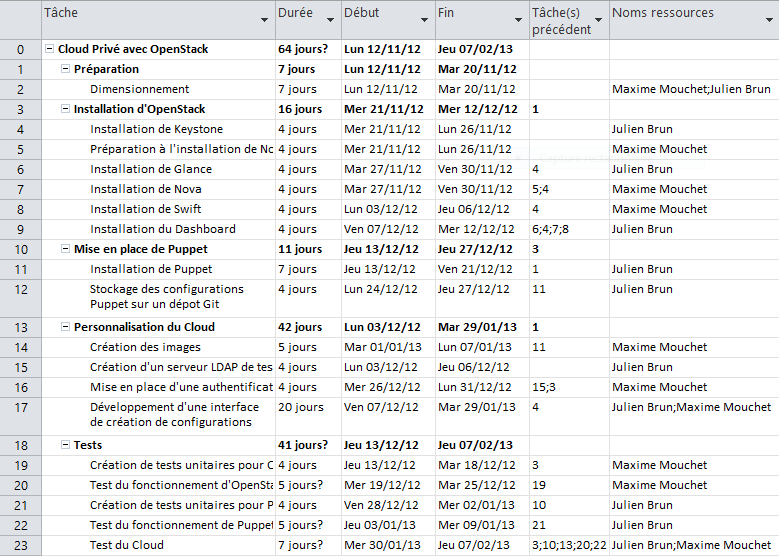
\includegraphics[width=19cm,angle=90]{images/liste.png}

\section{Liste détailée}
\subsection*{Tâche 2 : Dimensionnement}
\begin{description}
\item[Objectif :] Définir le matériel (nombre de machines) nécessaires
\item[Durée :]  1 semaine
\item[Assignée à :] Maxime Mouchet, Julien Brun
\end{description}

\subsection*{Tâche 4 : Installation de Keystone}
\begin{description}
\item[Objectif :] Installer et configurer le service de gestion d'identité et de l'API
\item[Durée :]  4 jours
\item[Assignée à :] Julien Brun
\end{description}

\subsection*{Tâche 5 : Préparation à l'installation de Nova}
\begin{description}
\item[Objectif :] Installer et configurer un système de virtualisation
\item[Durée :]  4 jours
\item[Assignée à :] Maxime Mouchet
\end{description}

\subsection*{Tâche 6 : Installation de Glance}
\begin{description}
\item[Objectif :] Installer et configurer le service de gestion des images
\item[Durée :]  4 jours
\item[Assignée à :] Julien Brun
\end{description}

\subsection*{Tâche 7 : Installation de Nova}
\begin{description}
\item[Objectif :] Installer et configurer le service de gestion des machines virtuelles
\item[Durée :]  4 jours
\item[Assignée à :] Maxime Mouchet
\end{description}

\subsection*{Tâche 8 : Installation de Swift}
\begin{description}
\item[Objectif :] Installer et configurer le service de stockage objet
\item[Durée :]  4 jours
\item[Assignée à :] Maxime Mouchet
\end{description}

\subsection*{Tâche 9 : Installation du Dashboard}
\begin{description}
\item[Objectif :] Installer et configurer l'interface web de gestion
\item[Durée :]  4 jours
\item[Assignée à :] Julien Brun
\end{description}

\subsection*{Tâche 11 : Installation de Puppet}
\begin{description}
\item[Objectif :] Installation de puppet master sur une machine et installation manuelle du client sur quelques instances virtuelles
\item[Durée :]  1 semaine
\item[Assignée à :] Julien Brun
\end{description}

\subsection*{Tâche 12 : Stockage des configurations Puppet sur un dépot Git}
\begin{description}
\item[Objectif :] Création d’un serveur Git, centralisation des fichiers de configurations
\item[Durée :]  4 jours
\item[Assignée à :] Julien Brun
\end{description}

\subsection*{Tâche 14 : Création des images}
\begin{description}
\item[Objectif :] Créer les images de machines virtuelles
\item[Durée :]  5 jours
\item[Assignée à :] Maxime Mouchet
\end{description}

\subsection*{Tâche 15 : Création d'un serveur LDAP de test}
\begin{description}
\item[Objectif :] Créer un serveur LDAP de test pour la tâche 16
\item[Durée :]  4 jours
\item[Assignée à :] Julien Brun
\end{description}

\subsection*{Tâche 16 : Mise en place d'une authentification via le LDAP}
\begin{description}
\item[Objectif :] Configurer Keystone pour utiliser un LDAP
\item[Durée :]  4 jours
\item[Assignée à :] Maxime Mouchet
\end{description}

\subsection*{Tâche 17 : Développement d'une interface de création de configurations}
\begin{description}
\item[Objectif :] Recherche d'une solution libre pour la création de fichiers de configurations. Sinon nous la développerons.
\item[Durée :]  20 jours
\item[Assignée à :] Julien Brun, Maxime Mouchet
\end{description}

\subsection*{Tâche 19 : Création de tests unitaires pour OpenStack}
\begin{description}
\item[Objectif :] Créer des tests automatisés pour OpenStack
\item[Durée :]  4 jours
\item[Assignée à :] Maxime Mouchet
\end{description}

\subsection*{Tâche 20 : Test du fonctionnement d'OpenStack}
\begin{description}
\item[Objectif :] Lancements des tests pour OpenStack et correction des problèmes si nécessaires
\item[Durée :]  5 jours?
\item[Assignée à :] Maxime Mouchet
\end{description}

\subsection*{Tâche 21 : Création de tests unitaires pour Puppet}
\begin{description}
\item[Objectif :] Crée des tests automatisées pour vérifier le bon fonctionement de Puppet
\item[Durée :]  5 jours?
\item[Assignée à :] Julien Brun
\end{description}

\subsection*{Tâche 22 : Test du fonctionnement de Puppet}
\begin{description}
\item[Objectif :] Lancements des tests pour Puppet et correction des problèmes si nécessaires
\item[Durée :] 5 jours?
\item[Assignée à :] Julien Brun
\end{description}

\subsection*{Tâche 23 : Test du Cloud}
\begin{description}
\item[Objectif :] Test global du système
\item[Durée :] 7 jours?
\item[Assignée à :] Julien Brun; Maxime Mouchet
\end{description}

\section{GANTT}
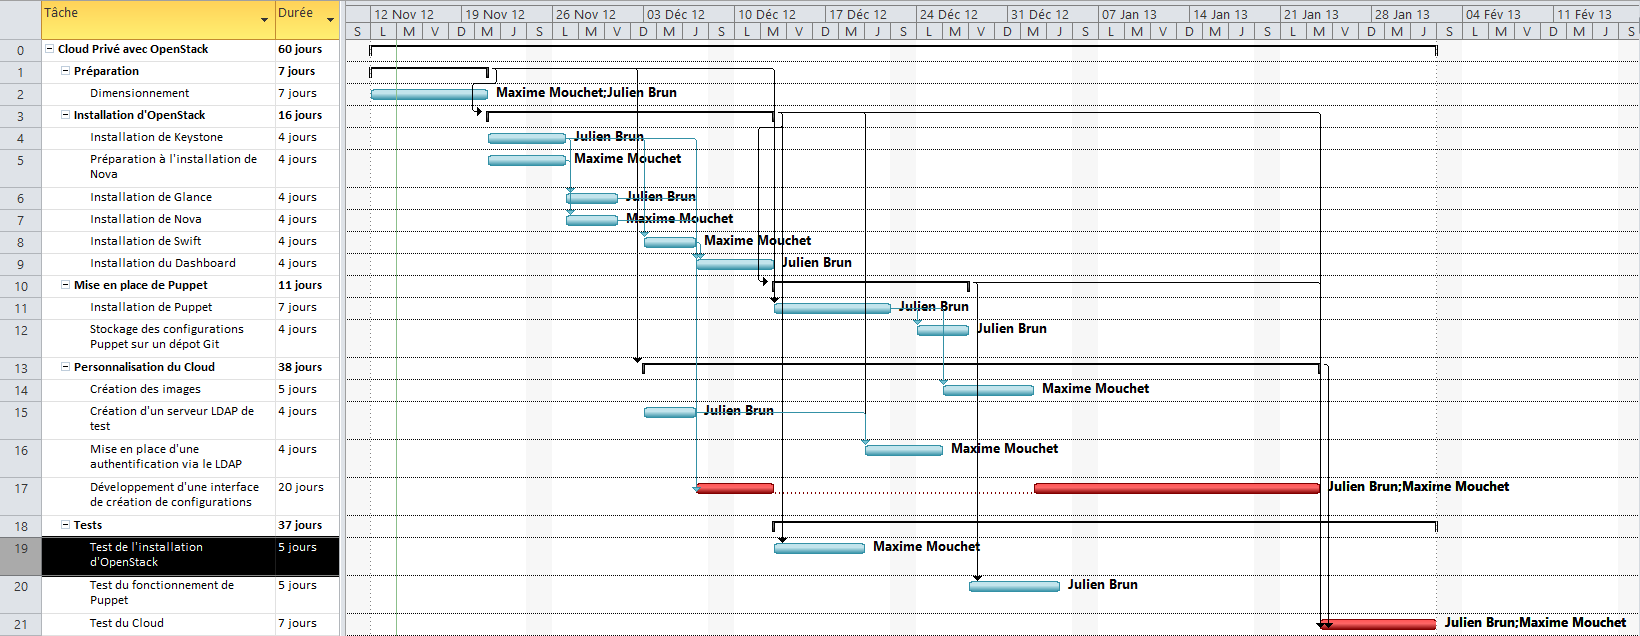
\includegraphics[width=25cm,angle=90]{images/gantt.png}

\section{Lexique}
\begin{description}
\item[Virtualisation :] Technique permettant de faire fonctionner plusieurs systèmes d'exploitations en simultanés sur une même machine physique.

\item[Cloud Computing :] Accès via le réseau, en libre-service, à des ressources informatiques virtualisées et mutualisées.

\item[IaaS :] Infrastructure as a Service. Niveau le plus bas du cloud computing où un fournisseur expose une infrastructure informatique (serveurs, stockage, réseau) au client. Le client ne gère que les systèmes d'exploitation et logiciels qui vont fonctionner dessus.

\item[OpenStack :] IaaS Open Source développé principalement par Rackspace (un grand hébergeur Américain) et la NASA.

\item[NAS :] Network Attached Storage. Système de stockage de grande capacité (plusieurs To en général) accessible via le réseau.

\item[SAN :] Storage Area Network. Semblable au NAS mais se caractérise pas un accès plus bas-niveau aux disques et donc à des performances accrues.

\item[VT-x :] Technologie incluse dans les processeurs récents permettant aux machine virtuelles d'accéder directement au processeur, ce qui permet d'augmenter les performances.

\item[KVM :] Kernel-based Virtual Machine. Système de virtualisation intégré dans le noyau Linux utilisant la virtualisation matérielle (VT-x) et donc très performant. Il est capable de faire fonctionner aussi bien des systèmes basés sur un noyau Linux, que BSD ou Windows.

\item[LXC :] Linux Containers. Système de virtualisation léger ne nécessitant pas VT-x au contraire de KVM ou Xen par exemple. Il ne supporte que les systèmes basés sur un noyau Linux. Semblable aux Jails de BSD.
\end{description}
 

\end{document}